%Notes by Harsh Mistry 
%Econ 301
%Based on Template From  https://www.cs.cmu.edu/~ggordon/10725-F12/template.tex

\documentclass[twoside]{article}
\setlength{\oddsidemargin}{0.25 in}
\setlength{\evensidemargin}{-0.25 in}
\setlength{\topmargin}{-0.6 in}
\setlength{\textwidth}{6.5 in}
\setlength{\textheight}{8.5 in}
\setlength{\headsep}{0.75 in}
\setlength{\parindent}{0 in}
\setlength{\parskip}{0.1 in}
\usepackage{amsmath,amsfonts,graphicx, color}
\newcounter{lecnum}
\renewcommand{\thepage}{\thelecnum-\arabic{page}}
\renewcommand{\thesection}{\thelecnum.\arabic{section}}
\renewcommand{\theequation}{\thelecnum.\arabic{equation}}
\renewcommand{\thefigure}{\thelecnum.\arabic{figure}}
\renewcommand{\thetable}{\thelecnum.\arabic{table}}
\newcommand{\lecture}[4]{
   \pagestyle{myheadings}
   \thispagestyle{plain}
   \newpage
   \setcounter{lecnum}{#1}
   \setcounter{page}{1}
   
   
%Info Box 
   \begin{center}
   \framebox{
      \vbox{\vspace{2mm}
    \hbox to 6.28in { {\bf Econ 301 - Microeconomic Theory 2
	\hfill Winter 2018} }
       \vspace{4mm}
       \hbox to 6.28in { {\Large \hfill Lecture #1: #2  \hfill} }
       \vspace{2mm}
       \hbox to 6.28in { {\it Lecturer: #3 \hfill Notes By: #4} }
      \vspace{2mm}}
   }
   \end{center}
   
   \markboth{Lecture #1: #2}{Lecture #1: #2}



 
}

\renewcommand{\cite}[1]{[#1]}
\def\beginrefs{\begin{list}%
        {[\arabic{equation}]}{\usecounter{equation}
         \setlength{\leftmargin}{2.0truecm}\setlength{\labelsep}{0.4truecm}%
         \setlength{\labelwidth}{1.6truecm}}}
\def\endrefs{\end{list}}
\def\bibentry#1{\item[\hbox{[#1]}]}

\newcommand{\fig}[3]{
			\vspace{#2}
			\begin{center}
			Figure \thelecnum.#1:~#3
			\end{center}
	}
	
	\graphicspath{ {images/} }

\newtheorem{theorem}{Theorem}[lecnum]
\newtheorem{lemma}[theorem]{Lemma}
\newtheorem{ex}[theorem]{Example}
\newtheorem{proposition}[theorem]{Proposition}
\newtheorem{claim}[theorem]{Claim}
\newtheorem{corollary}[theorem]{Corollary}
\newtheorem{definition}[theorem]{Definition}
\newenvironment{proof}{{\bf Proof:}}{\hfill\rule{2mm}{2mm}}
\newcommand\E{\mathbb{E}}


%Start of Document 
\begin{document}

\lecture{16}{March 12, 2018}{Jean Guillaume Forand}{Harsh Mistry}

\section{Welfare Continued}

\subsection{Second Welfare Theorem Continued}
\begin{center}
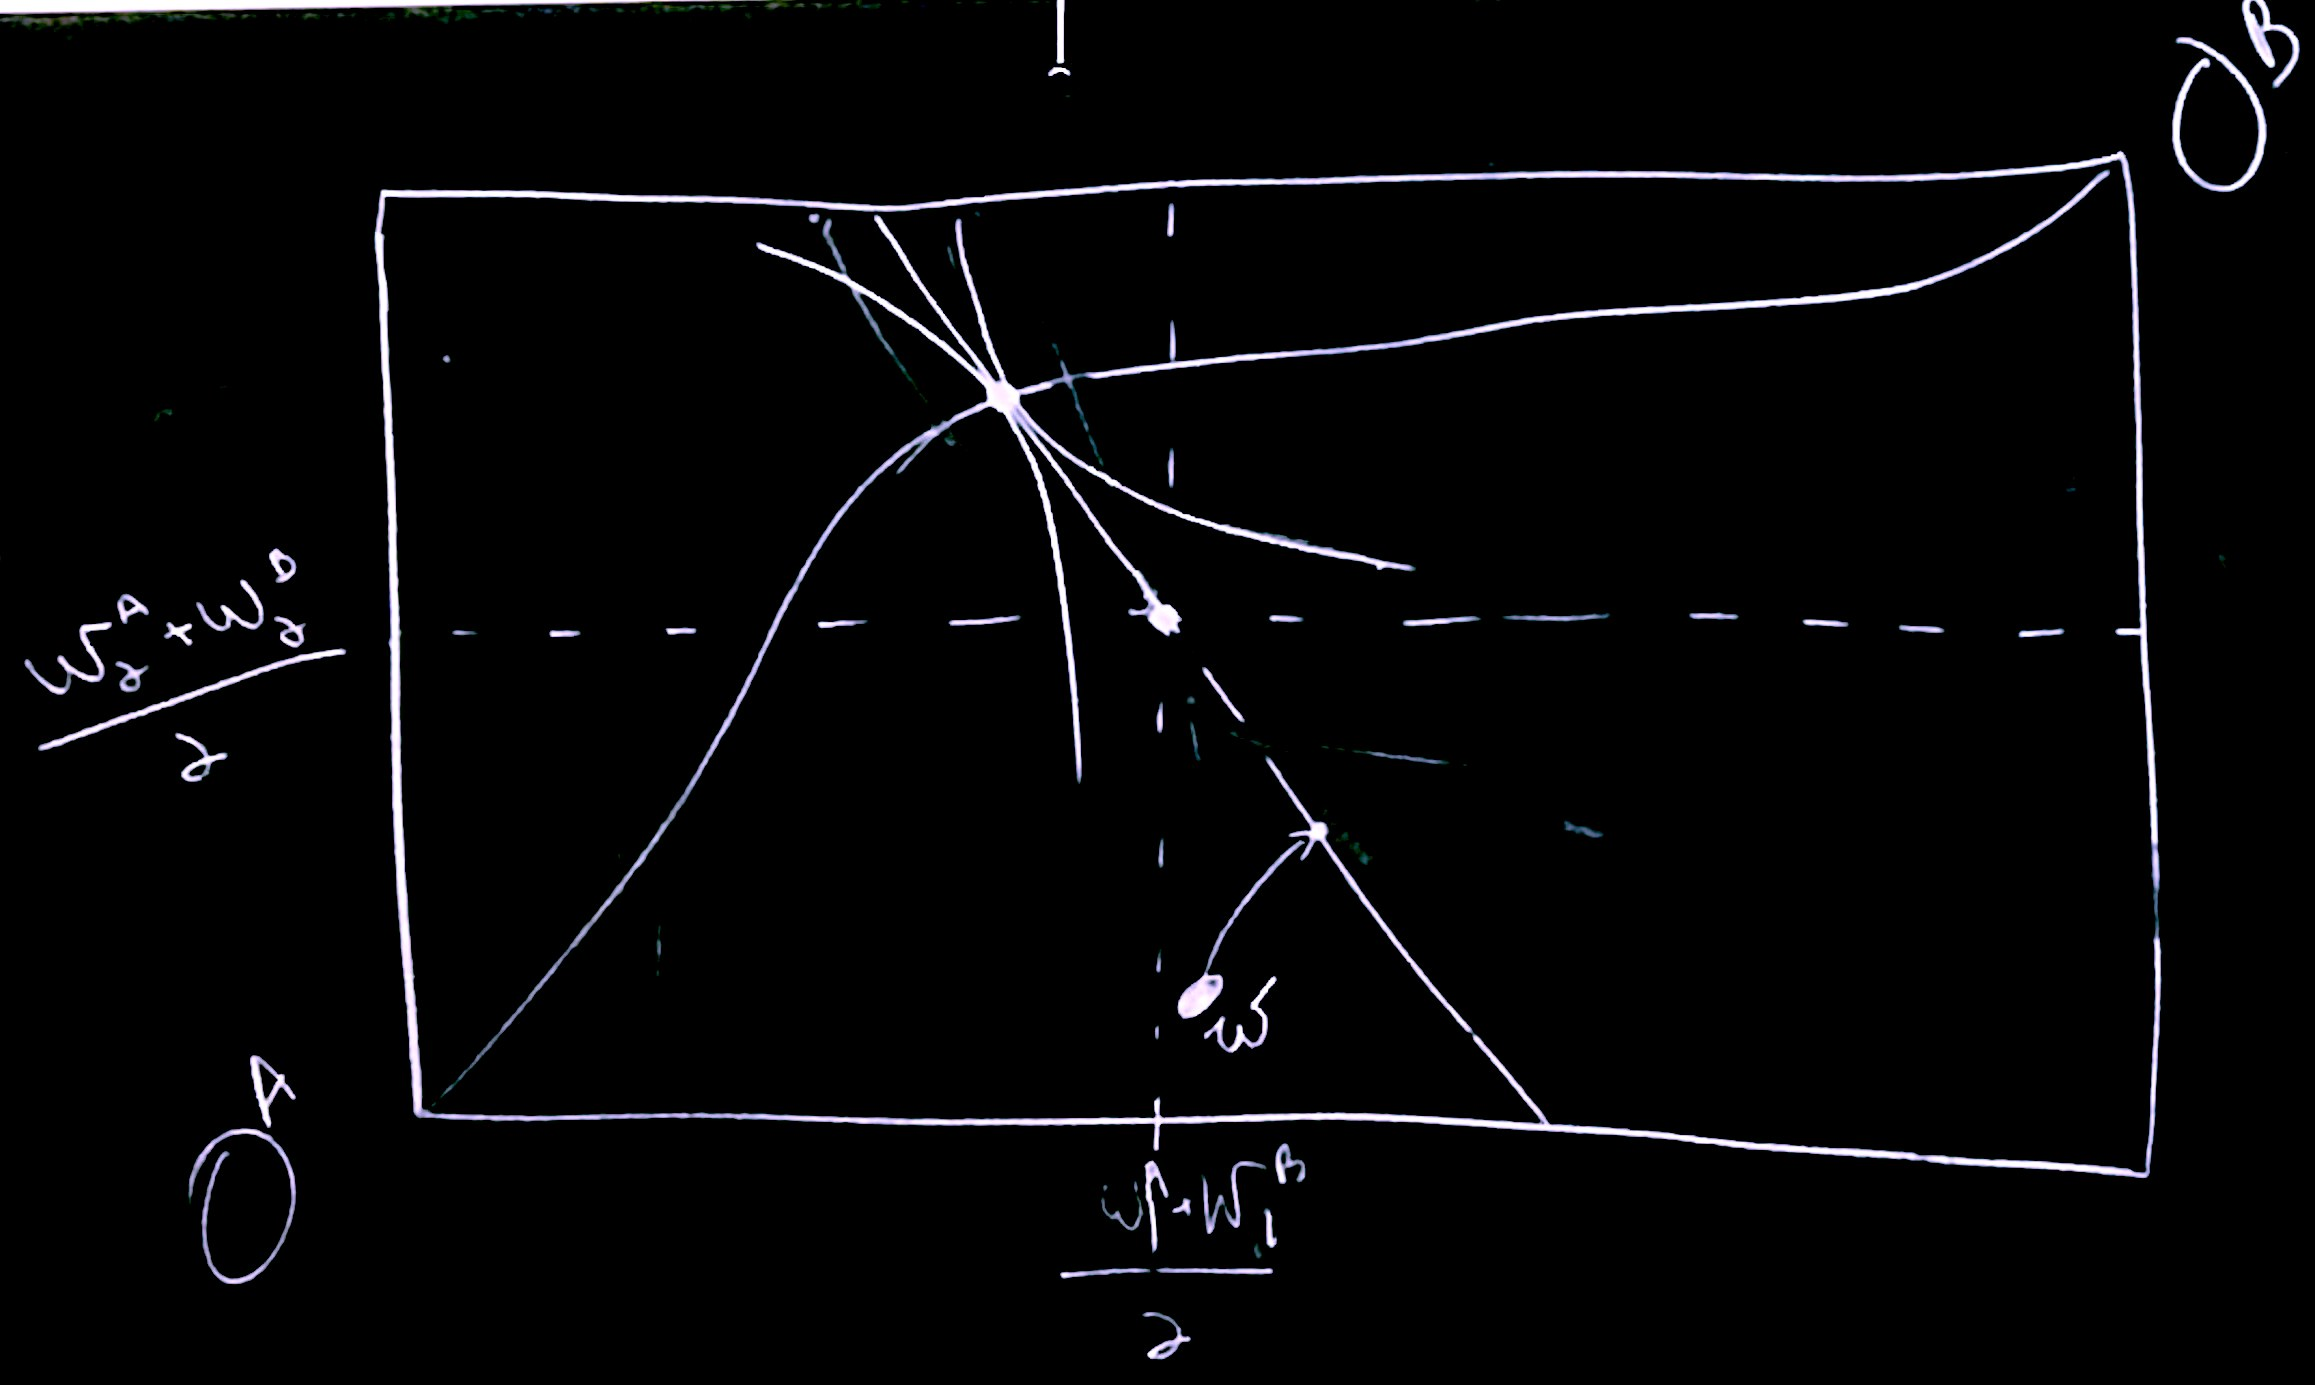
\includegraphics[scale=0.07]{29}
\end{center}
\begin{theorem}
(SWT) If consumers' preferences are monotone and convex, then for any Pareto-efficient allocations \(x^A\) and \(x^B\), there exists endowments \(\omega^A\) and \(\omega^B\) along with a competitive equlibrium that generates \(x^A\) and \(x^B\). 
\end{theorem}

\begin{itemize}
\item[\(\star\)] \textbf{FWT :} Competitive equilibrium which exhausts gains from trade
\item[\(\star\)] \textbf{SWT :} Competitive equilibrium which takes no stand on final distribution of goods.
\end{itemize}

\begin{itemize}
\item SWT leaves room for government intervention that is consistent with Pareto-efficiency
\begin{itemize}
\item Redistribution of endowments is a system of taxation. 
\item In the figure, endowment distribution entails increasing consumer A's endowment of good 2.
\end{itemize}
\item What if instead government subsidised consumption of good 2 by consumers A? 
\begin{itemize}
\item Given any equilibrium price \(p^*\), the price paid for good 2 by consumers A is \(p_2^* - s\) 
\item Any equilibrium allocations \(x^{A*}\) and \(x^{B*}\) are \underline{not} Pareto-efficient because 
\[\begin{aligned} & \frac{\frac{d}{dx_1^A} u^A(x_1^{A*}, x_2^{A*}) }{\frac{d}{dx_2^A} u^A(x_1^{A*}, x_2^{A*}) } = \frac{p_1^*}{p_2^* - s} & \hspace{0.2cm}(MRS_a)\\
& \frac{\frac{d}{dx_1^B} u^B(x_1^{B*}, x_2^{B*}) }{\frac{d}{dx_2^B} u^B(x_1^{B*}, x_2^{B*})} = \frac{p_1^*}{p_2^*} & \hspace{0.2cm} (MRS_b)
\end{aligned} \]

\end{itemize}
\item In summary, Redistribution of endowments does not affect consumers' marginal incentives. 
\item Subsidies ensure that consumer A values units of good 2 less that consumer B on equilibrium, so there are gains from trade between them.
\end{itemize}
\newpage
\section{Externalities} (Finally! Almost done with micro)
\textcolor{red}{In-class Numbering : 4.0}\\
\begin{itemize}
\item An allocation of competitive markets is their decentralization
\item A problem can arise, if consumption choices of some consumer impact well being of other consumer. This is called \underline{Consumption externalities}
\item  \underline{Positive externalities} are present if some consumers benefit from the consumption of a good by other consumers.  
\item Trivially, \underline{Negative externalities} are presentif some consumers do not benefit from the consumption of a good by others. 
\item In competitive markets, how do consumers' decisions internalise the effects they have on others?
\end{itemize}
\begin{center}
\textbf{To be continued next lecture.}
\end{center}


\end{document}





